\documentclass[10pt]{article}
\usepackage{page_style}

\usepackage{xcolor}
\definecolor{darkblue}{HTML}{00037D}

\usepackage{hyperref}
\hypersetup{
    colorlinks=true,
    linkcolor=darkblue,      
    urlcolor=darkblue,
    citecolor=darkblue,
}

\lstset{
  basicstyle=\footnotesize,
  xleftmargin=.2\textwidth, 
  xrightmargin=.2\textwidth
}

% %%%%%%%%%%%%%%%%%%%%%%%%%   COMMANDS   %%%%%%%%%%%%%%%%%%%%%%%%%%%%%%%%%
\newcommand{\ts}{\textsuperscript}
\newcommand{\maxnodes}{N_{max}}
\newcommand{\dth}{D_{threshold}}


\newcommand{\func}[1]{\path{#1()}}

\newcommand{\computedistances}{\func{compute_distances}}
\newcommand{\comparecombinations}{\func{_compare_combinations}}
\newcommand{\finddataregions}{\func{find_data_regions}}
\newcommand{\identifydataregions}{\func{_identify_data_regions}}
\newcommand{\finddatarecords}{\func{find_data_records}}
\newcommand{\findrecordsone}{\func{_find_records_1}}
\newcommand{\findrecordsn}{\func{_find_records_n}}

\newcommand{\gn}{\path{GNode}}
\newcommand{\dr}{\path{DataRegion}}
\newcommand{\drec}{\path{DataRecord}}
\newcommand{\nodenamer}{\path{NodeNamer}}

\newcommand{\citefootnote}[1]{\footnote{\cite{#1}.}}

% %%%%%%%%%%%%%%%%%%%%%%%%%   HEADER   %%%%%%%%%%%%%%%%%%%%%%%%%%%%%%%%%
\title{
    \huge Project Report: Mining Data Records in Python \\ 
    \medskip
    \large Data Wrangling with Leonid Libkin \& Pierre Senellart \\
    \medskip
    Master IASD - PSL University
}

\author{
    João Paulo Casagrande Bertoldo \\
    \href{mailto:joaopcbertoldo@gmail.com}{\texttt{joaopcbertoldo@gmail.com}} 
}
    
\date{April 2020}


% %%%%%%%%%%%%%%%%%%%%%%%%%   DOCUMENT   %%%%%%%%%%%%%%%%%%%%%%%%%%%%%%%%%

\begin{document}

% elements to mention
% - api 
% - extension
% - file management

% setup.py not been tested


% https://github.com/joaopcbertoldo/pymdr

% %%%%%%%%%%%%%%%%%%%%%%%%%   ABSTRACT   %%%%%%%%%%%%%%%%%%%%%%%%%%%%%%%%%
{
    \setstretch{.7} 
    \maketitle

    \begin{abstract}
    
    This project is part of the evaluation of the course \href{https://moodle.di.ens.fr/enrol/index.php?id=14}{Data Wrangling} with Professors Leonid Libkin and Pierre Senellart as part of the \href{https://www.lamsade.dauphine.fr/wp/iasd/en/}{Master's degree IASD} at the \href{https://www.psl.eu/en}{PSL University} (session 2019/2020).
    \medskip
    
    This report presents a review on my Python \href{https://github.com/joaopcbertoldo/pymdr/tree/0.1.1}{ implementation} of the algorithm \emph{Mining Data Records in Web Pages}, designed by \cite{mdr}. 

    \end{abstract}
}

\tableofcontents
\newpage

% %%%%%%%%%%%%%%%%%%%%%%%%%   BODY   %%%%%%%%%%%%%%%%%%%%%%%%%%%%%%%%%


\section{Introduction}

The initial goal of this project was to implement an open version of the algorithm created by \cite{mdr} in Python. In addition to it, the project aimed to include a visualization feature that would allow the user to inspect the code execution. Unfortunately, as we will see in Section \say{\nameref{txt:implementation}}, the algorithm did not work as expected at first. 

As a consequence, I changed the project's goals to investigate that and try to correct the problem by changing it's parameters. For this reason, the visualization was not implemented. Although, the final results are presented in a rudimentary version of that by coloring data records directly in the HTML pages.

I argue, based on my experiments, that this algorithm does not seem to work with today's websites. I experimented MDR's main parameter, the edit distance threshold, to show that. Besides, I show that, using \citeauthor{mdr}'s assumptions, today's pages do not even return results at all.

In the following sections, first, I summarize the original paper that introduced the algorithm \emph{Mining Data Records} (MDR), then I present the main components of my implementation, and finally explain how I tested it and what the results show. 

The project is stored in an open GitHub repository under the MIT License: \href{https://github.com/joaopcbertoldo/pymdr/tree/0.1.1}{link to the repository}. 



\section{Original Paper}

To implement this algorithm, I based myself on the paper \emph{Mining Data Records in Web Pages}, by \cite{mdr-technical}. According to Semantic Scholar\citefootnote{mdr-semantic-scholar}, it has been cited over $400$ times, of which more than $90$ articles were highly influenced by it.



\subsection{Authors}

\paragraph{Bing Liu}

is a Distinguished Professor of Computer Science at the University of Illinois at Chicago (UIC). He published many articles, like the one used for this project, about data mining applied to data from the web and wrote of the book \emph{Web Data Mining} \citep{web-data-mining}.\citefootnote{liu-page}

\paragraph{Robert L. Grossman}

was a professor at the University of Illinois at Chicago for more than 20 years. Nowadays he is a professor at the University of Chicago. Grossman has received several awards and makes part of a number of advisory boards. He is Chair of the Open Commons Consortium (OCC) and ACM Fellow since 2016.\citefootnote{robert-page, robert-linkedin}

\paragraph{Yanhong Zhai}

was, by the time of the publication, a Ph.D. student at the University of Illinois at Chicago. Since her Ph.D. degree in 2006, Yanhong has been working in Microsoft as Software Development Engineer (SDE) for more than 10 years. Notably, she has worked in web data mining and is now a Principal SDE in the company. \citefootnote{yanhong-page, yanhong-linkedin}



\subsection{Overview}

The article introduces and explains the algorithm \emph{Mining Data Records} (MDR). A \emph{data record} is a structured object on a page that holds information about some entity. The latter can be, supposedly, from a database of records exposed on the website. For instance, it can be a product on a market place website like Amazon (Figure \ref{fig:pianos}).

\begin{figure}[!t]
  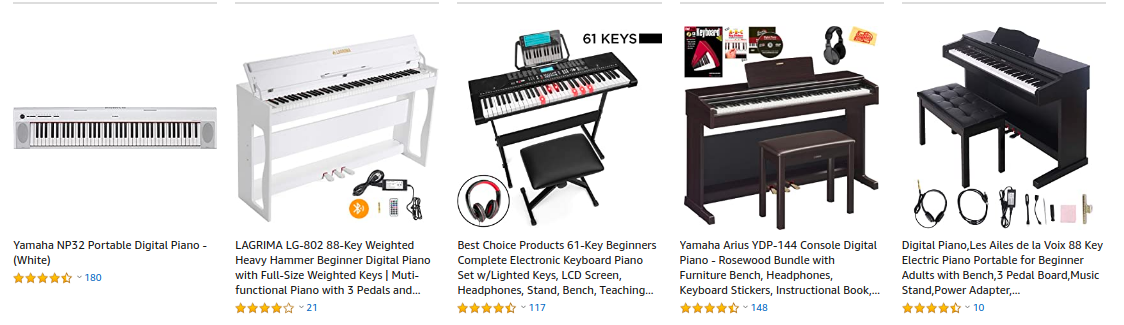
\includegraphics[width=0.9\linewidth]{fig/pianos.png}
  \caption{Sample page from \href{www.amazon.com}{www.amazon.com} with data records about pianos. Each product offered on the page is a data record - that is, an object containing an image, a title, a rating, and the number of purchases of the product.}
  \label{fig:pianos}
\end{figure}

MDR finds data records inside table tags in HTML pages without using any heuristics about the page's contents or topic. Here below, I briefly describe the article's contents, but the reader is encouraged to read the short \citep{mdr} or technical \citep{mdr-technical} version of the original publication for more details.

\paragraph{Rationale}

Consider an HTML document as a tree structure where tags inside another are children of the latter (see Figure \ref{fig:html-as-tree}). The core of the algorithm is based on three ideas: the notion of Generalized Node (noted \gn{} for short), Data Region (noted \dr{}), and a measure of the distance between \gn{}s. 

A \gn{}  is a set of $n \in \{1, ..., \maxnodes\}$ adjacent nodes (thus, under the same parent node). A \dr{} is a sequence of adjacent \gn{}s that are \emph{similar}. See Figure \ref{fig:gnode-and-dr} for an illustration of these two concepts. In this context, \emph{similar} means that the distance between each two directly adjacent \gn{}s is less than the threshold $\dth$. The measure of distance is the Normalized Levenshtein Edit Distance \footnote{See the \cite{lev-dist-wiki} for more information.}:

\begin{equation}\label{eq:dist}
    d\left(s_{1}, s_{2}\right)=\frac{LevenshteinEditDist\left(s_{1}, s_{2}\right)}{\frac{\text {length}\left(s_{1}\right)+\text {length}\left(s_{2}\right)}{2}} \in [0, 1]
\end{equation}

The values of $\maxnodes$ and $\dth$ are parameters of the algorithm and the authors reported using, respectively, $10$ and $0.30$. Once the \dr{}s are found in the HTML, there is a scan over them that figure out where the data records are.


\begin{figure}[!b]
    \centering
    
    \begin{subfigure}[b]{.39\textwidth}
        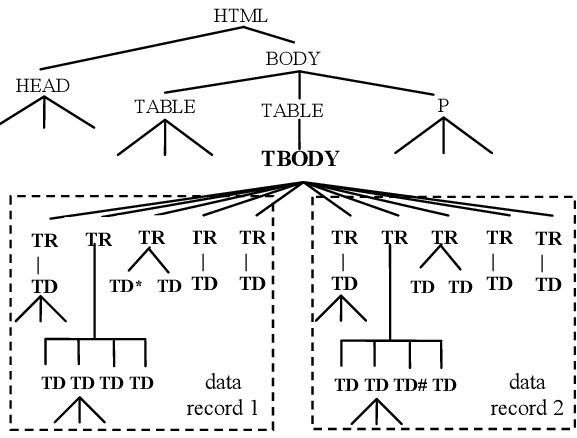
\includegraphics[width=0.95\linewidth,left]{fig/html-as-tree.png}
        \caption{HTML as a tree structure.}
        \label{fig:html-as-tree}
    \end{subfigure}
    %
    \begin{subfigure}[b]{.60\textwidth}
        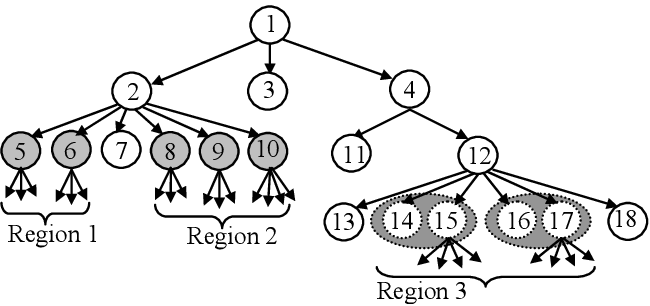
\includegraphics[width=0.95\linewidth,right]{fig/gnode-and-dr.png}
        \caption{\gn{} and \dr{} concepts illustrated. Region 1 is a \dr{} with two \gn{}s of size $n = 1$. Region 2 is a \dr{} with three \gn{}s of size $n = 1$. Region 3 is a \dr{} with two \gn{}s of size $n = 2$. }
        \label{fig:gnode-and-dr}
    \end{subfigure}
    
    \caption{Key concepts. Source: \cite{mdr}.}
    \label{fig:html-gnode-dr}
\end{figure}


\paragraph{Experimental results}

The authors tested MDR on $46$ different pages, with a total of $621$ objects (data records). They reported precision and recall of, respectively, $100\%$ and $99.8\%$, outperforming (by far) other previously proposed algorithms. The list of websites used by them can be seen in Table 1 in \cite{mdr}. 

\paragraph{Issues}

Unfortunately, the authors did not make available any reference implementation. They also did not make public the specific cached HTML pages that they used to test the algorithm on, or even the specific URLs of the pages used (only the websites). Some of the websites mentioned in their test set do not exist anymore (like \href{http://www.bookbuyer.com}{\textit{bookbuyer.com}} and \href{http://www.codysbooks.com}{\textit{codysbooks.com}}) or became a completely different website (such as \href{https://www.eveonline.com/}{\textit{eveonline.com}}). Moreover, they do not describe how the data was labeled or inspected, making it hard to reproduce their metrics.



\section{Implementation} \label{txt:implementation}

\subsection{Overview}

The first implementation of the algorithm, with the suggested parameters, did not work as the authors claim. For this reason, I decided to investigate the effect of some parameters and variations of the algorithm. To test my implementation, I collected HTML pages and annotated the number of data records in each of them. To facilitate the annotation task, I created a Google Chrome extension to interface with a Flask\footnotemark web API. Next, I ran the algorithm's steps individually, saving intermediate results for inspection.

\footnotetext{\href{https://flask.palletsprojects.com/en/1.1.x/}{Link to Flask's official page}.}

% implementation + viz...
% core, utils, api
\paragraph{Code structure} The next subsections will explain the main components (modules, classes, functions, etc) of my code. (Most of) The code referenced in this section is organized in the following structure\footnotemark:

\footnotetext{\href{https://github.com/joaopcbertoldo/pymdr}{Link to the \emph{pymdr} project GitHub repository}.}

\begin{lstlisting}[caption=Main code structure.]
# project root
/  
|--/src
|  |--/api
|  |  |-- main.py
|  |  
|  |--/extension
|  |  |-- readme.txt
|  |  |-- manifest.json
|  |   ...
|  |
|  |-- core.py
|  |-- files_management.py
|  |-- prepostprocessing.py 
|  |-- utils.py
|
|--/test 
|   ...
|
|--/dev
|  |--/training
|  |  |-- evaluating_stuff-with-list.ipynb
|  |  |-- evaluating_stuff-with-list-with-cleanup.ipynb
|  |  |-- evaluating_stuff-withOUT-list.ipynb
|  |  |-- evaluating_stuff-withOUT-list-with-cleanup.ipynb
|  |  |-- preprocess_all.py
|  ...
\end{lstlisting}



\subsection{Core}

This is where the algorithm itself and the entities (classes) that interact with it live. The code in this module is not supposed to manage any of the files, inputs or outputs formats, nor treat the way they are loaded and saved. Instead, it expects all the inputs to be in known specific formats.

The main input types are \path{HtmlElement} (from \path{lxml.html}), the classes defined in the module (discussed next), and a few dictionary structures, which are specified with \path{typing}\footnotemark for documentation\footnotemark.

\footnotetext{\href{https://docs.python.org/3.6/library/typing.html}{Link to the \path{typing} library's page in Python 3.6}.}

\footnotetext{\href{https://github.com/joaopcbertoldo/pymdr/blob/7ff7f7653feff23704b6b786db8499188ba378af/src/core.py\#L273}{Link to their definitions in \path{core.py} in the repository}.}



\subsubsection{Dependencies}

\paragraph{\path{lxml}} 

After reading about\footnotemark and experimenting with a few Python libraries for HTML handling, I chose \path{lxml} for a few reasons. First, it is designed to work with the \path{ElementTree} API, making it simple to treat HTML documents as a tree structure like the original paper does. Second, it is fairly easy to parse the HTML into \path{HtmlElement} and serialize it back, which are the main functionalities I used. And finally, unlike other libraries, it is not full of fancy features that I did not need.

\footnotetext{For instance, \href{https://tomassetti.me/parsing-html/\#python}{this review on \emph{tomassetti.me}}.}

\paragraph{\path{graphviz}} Since the original goal was to generate visualizations, I also reviewed several options for graph rendering and chose \path{graphviz} because it is open source. Also, it provides a fairly simple interface for the features I was looking for. In the end, it was not used in the core code, but you may find some utility functions that can be used to render a graph from an \path{HtmlElement}.

\paragraph{\path{python-Levenshtein}} One of the core tasks in the algorithm is to measure the (normalized) Levenshtein edit distance between strings - remember that \gn{}s are \emph{similar} if this distance is below a threshold. I initially used the library \path{strsim}\footnotemark, but it started creating problems (which I could not debug) at some point. So I switched to the library \path{python-Levenshtein}\footnotemark.

\footnotetext{\href{https://pypi.org/project/strsim/}{Link to \path{strsim}'s PiPy page}.}

\footnotetext{\href{https://pypi.org/project/python-Levenshtein/}{Link to \path{python-Levenshtein}'s PiPy page}.}



\subsubsection{Classes} \label{txt:classes}

\paragraph{\gn{}}

corresponds exactly to the concept of \emph{Generalized Node} introduced in the original paper. It represents a set of subsequent HTML tags in the document graph and it includes all the subtrees starting at its nodes. In practice, it is referenced by its parent's name and the (0-starting) indices of the first and last HTML tags of the \gn{}.

\paragraph{\dr{}} 

is a tuple with the \gn{} size $n$ (i.e. the number of HTML tags in it), the index of the first tag of the first \gn{}, and the number of tags covered by the \gn{}. This notation is not very intuitive but it is handy inside the algorithms that use it. For practical reasons, I also added to it the parent's name - which is, by definition, the same as its covered \gn{}s' parent. 

\paragraph{\drec{}} \label{txt:class-data-record} 

Most of the time, \drec{}s correspond exactly to one \dr{}. However, some data records might be split into more than one \dr{}. For instance, when the titles of the objects are in cells of a table row and the description is in the respective cells of the next row\footnotemark. Therefore, a \drec{} object is defined as a list of \gn{}s, so both cases can be treated uniformly.

\footnotetext{This particular type of case is better explained in Section \emph{Non-contiguous object descriptions} in \cite{mdr}}

\paragraph{\nodenamer{}} 

Unfortunately, \path{lxml}'s implementation does not have a consistent \path{id()} (same for \path{__hash__()}). I do not know the reason, but I empirically checked that an \path{HtmlElement} object can return different values from those functions between calls (during the same run time). For this reason, it is not easy to uniquely reference any node of a generic HTML document. This limitation is crucial because the intermediate data structures (see the next section) map partial results per node. My solution was to add a node name as a tag attribute to the \path{HtmlElement}s of the document with a sequential value. The \nodenamer{} object serves as a stateful function that is used as a shortcut to get that value from the \path{HtmlElement}s - avoiding a snippet repetition and making it consistent.

\paragraph{MDR} 

puts together all the pieces of the algorithm (written in functions). It makes it easier to access some variables and mappings (the data structures described below) that are passed between the functions.

\paragraph{Others} 

During my tests, I considered using different distance thresholds in the different places where this notion is used (there are three of them). The class \emph{MDREditDistanceThresholds} would be used to allow this change to be made easily, but in the end, it was not used. Finally, \emph{WithBasicFormat} is a utility for printing the other data structure in a more readable way.



\subsubsection{Intermediate structures}

These two are important data structures for understanding the code because they act like mappings of information. They are used to pass sub-results between the sub-algorithms.

\paragraph{\path{DISTANCES_DICT_FORMAT}} It keeps all the distances between pairs of \gn{}s, which are computed before being used. This dictionary's keys are the node names and it maps a node to another dictionary. The latter maps the possible \gn{} sizes $n$ (integers from $1$ up to $\maxnodes$) to yet another dictionary. This last one maps pairs of \gn{} to distances (a float between $0$ and $1$). See the example below.

\begin{lstlisting}[caption=Illustration of a \path{DISTANCES_DICT_FORMAT}.]
{
    # node name
    "table-00000": {
        # GNode size
        1: {
            # GNode pair
            (
                GNode("table-00000", 0, 1), 
                GNode("table-00000", 1, 2)
            ): 0.1,
            
            (GNode(..., 1, 2), GNode(..., 2, 3)): 0.2,  # the distance
            (GNode(..., 2, 3), GNode(..., 3, 4)): 0.5,
            # ...
        },
        2: {...},
        # ...
        10: {...},
    },
    "table-00001": {...},
    "tr-00000": {...},
}
\end{lstlisting}


\paragraph{\path{DATA_REGION_DICT_FORMAT}} This one maps the nodes' names the set of \dr{}s found under that node.

\begin{lstlisting}[caption=Illustration of a \path{DISTANCES_DICT_FORMAT}.]
{
    # node name
    "table-00000": set({
        DataRegion("table-00000", 2, 0, 4),
        DataRegion("table-00000", 3, 6, 9),
    }),
    "table-00001": set({...}),
    "tr-00000": set({...}),
}
\end{lstlisting}



\subsubsection{Functions} \label{txt:functions} 

The main functions correspond almost exactly to the pseudo-codes described in the original paper. Their behaviors can be summarized as follows:

\begin{itemize}
    
    \item \computedistances: recursively iterates over all the nodes to compute the distances dictionary;
    
    \item \comparecombinations: on a given node, effectively goes through all the possible combinations of pairs of \gn{}s of all sizes and computes the distances;
    
    \item \finddataregions: recursively find all the data regions under a subtree of HTML document;
    
    \item \identifydataregions: on a given node, find all the data regions such that each one is the largest (in terms of covered nodes) possible; 
    
    \item \finddatarecords\footnotemark: scans all the\dr{}s to extract \drec{}s accordingly to two different cases: when the \gn{} sizes are of size 1 or larger;
    
    \footnotetext{This algorithm is not directly given in the paper like the other, but only described in the text.}
    
    \item \findrecordsone: creates \drec{}s either from all the \gn{} s of the \dr{} or from its children;
    
    \item \findrecordsn: creates \drec{}s directly from the \gn{}s covered by the \dr{} or from pieces of them to handle the case where the records are not contiguous (see the paragraph about the \nameref{txt:class-data-record} class).
    
\end{itemize}



\subsubsection{Parameters}

The algorithm has three parameters that are passed to the initialization of the MDR object:

\begin{itemize}
    
    \item \textbf{\path{minimum_depth}}: all nodes with a tree depth\footnote{\href{https://en.wikipedia.org/wiki/Tree-depth}{Link to the definition of "Tree depth" on Wikipedia}.} are not taken into consideration in the recursive calls of the functions described above. As a consequence, any direct child of these nodes can never be part of a \drec{};
    
    \item \textbf{max\_tag\_per\_gnode} ($\maxnodes$): the largest \gn{}  size taken into consideration;
    
    \item \textbf{edit\_distance\_threshold}: the maximum distance between two \gn{} s for them to be considered \emph{close} - therefore, possibly in the same \dr{}.
    
\end{itemize}




\subsection{Web API and Chrome Extension}

To make it easier to use and test \emph{pymdr}, I developed a minimalist Google Chrome extension that allows the user to call the algorithm on a (locally running) Flask API. The extension has two functionalities:  

\begin{enumerate}
    
    \item It copies and sends to the API the URL of the currently open page (button \emph{analyze}). Then the API executes the algorithm and returns a local file path (button \emph{copy output path}). The file is a local copy of the HTML page with all data records painted with different colors.
    
    \item The user inputs the correct number of data records on the page (input box \emph{nDataRecords}) and the API saves it (together with the page's URL) locally.
    
\end{enumerate}

The extension must be installed using Chrome's developer mode on and the API must be running locally. To install the extension, follow the instruction in the \path{readme.txt} file inside the extension's folder\footnotemark. To start the API, launch the script \path{launch-me.sh} in the root of the project\footnotemark.

\footnotetext{\href{https://github.com/joaopcbertoldo/pymdr/blob/0.1.1/src/extension/readme.txt}{Link to the extension's \path{readme.txt} file in the repository}.}

\footnotetext{\href{https://github.com/joaopcbertoldo/pymdr/blob/0.1.1/launch-api.sh}{Link to the \path{launch-me.sh} file in the repository}.}

\begin{figure}[H]
    \centering
    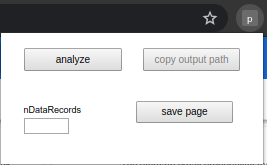
\includegraphics[width=0.45\linewidth]{fig/pymdr-extension.png}
    \caption{Screenshot of the Pymdr Google Chrome extension.}
    \label{fig:chrome-extension}
\end{figure}



\subsection{Other modules} \label{txt:other-modules}

The other two modules are rather for support tasks like managing files and treating the HTML files. They are mostly used in the API and in the script \path{preprocess_all.py} (explained in Section \say{\nameref{txt:procedure}}). 

\paragraph{\path{files_management}} 

defines utilities to write and read from files easily and keeping their locations consistent. The organization of the files mostly depends on the class \path{PageMeta}, which is used to access metadata from an annotated page. The files corresponding to a given page are referenced by a (shortened) hash of the URL where the page comes from. They are all located in the directory \path{outputs} at the root of the project. This directory's location can be changed in the file \path{config.yml} in the root of the project.

\paragraph{\path{prepostprocessing}}

wraps each sub-algorithm that compose MDR (see Section \nameref{txt:functions}). They save intermediate results in files, load them from previous steps, and ensure that the files already processed are skipped. This is useful to keep executions consistent between calls, especially in the script (see \say{\nameref{txt:procedure}}) used to process all the pages.



\subsection{Unit tests}

The directory \path{test} has the same structure as \path{src} and the respective files contain unit tests for those in the latter (see the Listing 1). They use Python's builtin package \path{unittest}. For maintenance purposes, I did not create unit tests for everything, but only for the most important parts of the algorithm. They were indeed very useful during my iterations of the code making sure to keep the code correct. These tests have rather simple input/output tests. So, it might be a useful entry point to understand those functions' interfaces. 



\section{Experiments}

From the very beginning, I realized it would be painful to test and inspect the results by managing the inputs and outputs of the core module manually. For this reason, I wrote the first version of the extension and the API only for caching the HTML pages, executing MDR, and returning another file with colored HTML tags to identify the data records.

\paragraph{(Very) Slow first results} 

My very first tests showed that my code was extremely slow. Although I did not record execution times, the typical execution time was in the tens of seconds (or even minutes). This is way above the authors' claims of sub-second execution times.

After re-reading the technical paper carefully, I realized that the algorithm is only supposed to consider table-related tags (table, tr, th, td, ...). In addition to that, the results did not seem correct at all. The algorithm was not capable of identifying any data record. This made sense because the algorithm was simply not intended to work with all the tags. 

I then started ignoring all other tags. It vastly accelerated the execution to a few seconds in the worst case. However, many of the pages did not have any data records at all. After manually inspecting a few, I realized that many of the pages simply did not use table tags, but lists (\path{<ol>} and \path{<ul>}) for organizing the data records. 

I hypothesize that web pages, today, use table tags way less often than when the algorithm was developed. According to \cite{tables-basics}: \say{...a lot of people used to use HTML tables to lay out web pages...}. This essentially breaks the algorithm because it is made to work well with these tags. Therefore, I decided to make sure it was not a matter of bad parameters. So I tested the algorithm with different threshold values since this is the most important parameter. 



\subsection{Analyzed factors} \label{txt:analyzed-factors}

\paragraph{Threshold}

The original recommended value was $0.30$, so it makes sense to keep the threshold range \emph{around} $0.30$. Also, the slowest part of the algorithm is (by far) the computation of the distances (see \nameref{txt:functions}). Fortunately, it does \textbf{not} dependent on the threshold choice. So, having a large value set for this parameter should not increase much the execution of the tests. Therefore, I tested with all the values in ${0.05, 0.06, ..., 0.49, 0.50}$.

\paragraph{HTML Lists} 

MDR was designed to work with table tags, so considering all the HTML tags did not make any sense. On the other hand, considering only tables seemed too restrictive (it will be explained in Section \nameref{txt:results}). Thus, I considered a version only with tables and another with lists additionally. This behavior can be controlled by changing the function \path{should_process_node}\footnotemark in \path{core.py}.

    \footnotetext{\href{https://github.com/joaopcbertoldo/pymdr/blob/258a195cd6481a2a6518edd64d1c79ffbcd31aea/src/core.py\#L1144}{Link to the function \path{should_process_node} in the repository}.}

\paragraph{Edit distance distortion}

While reviewing and cleaning my code, I realized that I introduced an issue to the algorithm by distorting the edit distances. This happened due to the naming solution I used to reference the nodes (see the class \nodenamer{} in Section \nameref{txt:classes}). It adds a new attribute to the HTML tags, so, while serializing subtrees, this attribute ends up as part of the string. This affects the distance measure especially for nodes with little content because the sizes of the attribute's key and value make the distances decrease artificially. 

For this reason, I made a hotfix that cleans all the attributes from the subtrees before measuring the distances. The parameter used to control this behavior is the constant \path{STR_DIST_USE_NODE_NAME_CLEANUP}\footnotemark  in \path{core.py}.

    \footnotetext{\href{https://github.com/joaopcbertoldo/pymdr/blob/258a195cd6481a2a6518edd64d1c79ffbcd31aea/src/core.py\#L31}{Link to the constant \path{STR_DIST_USE_NODE_NAME_CLEANUP} in the repository}.}

Therefore, there are four tests, corresponding to the combinations of the two previous parameters' values: $\{\text{with lists}, \text{without lists}\} \times \{\text{with correction}, \text{without correction}\}$. Here, \emph{correction} refers to the distance distortion hotfix. For each of these combinations, all the threshold values are tested. Then, I looked up for the best values and inspected \emph{promising} results manually in detail.



\subsection{Procedure} \label{txt:procedure}

\paragraph{Test pages}

First, I collected sample pages from the same websites mentioned in \cite{mdr}\footnotemark. Several of them did not exist or completely changed domain/content. In total, I collected $94$ pages, of which $86$ were processed - the others went through some problems in the process. 

    \footnotetext{I looked for the original cached pages used by the authors and even tried to get in touch with them to find them. Unfortunately, I could not find them out. I also tried to look up for the pages used in the two main references of the paper (OMNI and IEPAD), but they are also not available.}

I collected these pages using the Chrome extension to annotate the ground truth number of data records of each page. The pages' URLs and their annotations can be seen in the file \path{outputs/pages-meta.yml}\footnotemark.

    \footnotetext{\href{https://github.com/joaopcbertoldo/pymdr/blob/0.1.1/outputs/pages-meta.yml}{Link to the file \path{pages-meta.yml} in the repository}.}

\paragraph{Script}

I used the script \path{dev/training/preprocess_all.py}\footnotemark to go through all the thresholds, all the pages, step by step. To control the other parameters, one should directly change the code in \path{core.py}. It is possible to choose, directly in the script, which steps should be executed to avoid useless executions when running it multiple times.

    \footnotetext{\href{https://github.com/joaopcbertoldo/pymdr/blob/0.1.1/dev/training/preprocess_all.py}{Link to the script \path{preprocess_all.py} in the repository}.}
    


\paragraph{Outputs}

The results and intermediate files generated by the script are organized in the folder \path{outputs} under the root of the project. It contains the following subdirectories: 

\begin{itemize}

    \item \path{raw_htmls}: contains the cached HTML pages without any modification;
        
    \item \path{preprocessed_htmls}: contains HTML files after two phases of preprocessing: (1) without comments, script, and style tags; (2) with the node names added to all the tags (see \nodenamer{} in Section \say{\nameref{txt:classes}}).
        
    \item \path{intermediate_results}: contains two types of file: (1) the precomputed distances, returned by the function \computedistances{}; (2) the precomputed \dr{}s, whose files are separated by different threshold values\footnotemark because this parameter directly impacts the results.
    
        \footnotetext{Values are rounded up to two decimal places.}

    \item \path{results}: contains the \drec{}s in separate files following the same logic of the \dr{} files (i.e. by threshold value). It may also contain HTML files where the background of the tags in the same \drec{} are of the same color for inspection.
    
\end{itemize}

\paragraph{Reproduction}

All the result files can be found in the file \path{outputs/bkps-all.zip}\footnotemark. To inspect them, extract everything to \path{outputs}. You will see four directories starting with \say{bkp}. They correspond to the four different cases tested. 

\footnotetext{\href{https://github.com/joaopcbertoldo/pymdr/blob/0.1.1/outputs/bkps-all.zip}{Link to the file \path{bkps-all.zip} in the repository}.}

There are four Jupyter Notebooks inside \path{dev/training}. Again, they correspond to the combinations of parameters. They have all been executed with the parameters indicated in the files' names (also indicated in their first cells). To execute them, move the two directories inside one of the backup directories (\path{intermediate_results} and \path{results}) to \path{outputs}. I recommend looking, first, at \path{evaluating_stuff-with-list-with-cleanup.ipynb}\footnotemark because it is better commented with explanations. All the others have the same code but were not as much documented.

\footnotetext{\href{https://github.com/joaopcbertoldo/pymdr/blob/0.1.1/dev/training/evaluating_stuff-with-list-with-cleanup.ipynb}{Link to the file \path{evaluating_stuff-with-list-with-cleanup.ipynb} in the repository}.}


The reader can also easily rerun all the tests by executing the script in \path{dev/training/preprocess_all.py}. Please, note that the instructions in the \path{README.md} file should be followed before. Make sure that you empty the \path{outputs} folder before executing (except for the \path{pages-meta.yml}). You should also verify which steps of the process should be executed by setting the boolean parameters of the function \func{main} inside the script. 



\subsection{Evaluation}

\paragraph{Partial annotations} Since the task of manually annotating the data records inside each HTML file would have been too laborious, I opted for another solution. As mentioned before, I only annotated the correct number of data records on the pages, which is relatively easy to execute. For instance, see \href{https://www.circuitcity.com/products/health-personal-care-beauty.html}{\textit{this page}}: it has 12 records. Note that, if the algorithm finds 12 data records, it does not necessarily mean that it worked. The results might be in a completely different part of the HTML page that does not have any data record \emph{de facto}.

\paragraph{Simplification assumption} However, if it does not have 12 records in the results (or, say, 'almost'), it probably did not find the correct records. This is a reasonable assumption because the data records are usually adjacent. Therefore, finding the correct region should entail finding the other ones as well. An exception might occur when there is a disconnected data record\footnotemark.

\footnotetext{See Section \say{3.4 Data Records not in Data Regions} in \cite{mdr} for further detail}

Therefore, we will assume that this \emph{soft} annotation can be used as a valid way to check if the algorithm is working properly. Besides, it is laborious to inspect raw HTML. This framework was also useful to filter out bad candidates (e.g. eliminating cases with 60 data records where there should be 10) to inspect the good ones in detail.

% - no precise description of tagging/labelling --> how to measure precision/recall? --> simplified way of counting to investigate --> coloring the background for visual inspection

\paragraph{Visualizations} 

Since it is not reliable to compute accuracy metrics on this signal, I manually inspected many results and generated several visualizations to find good candidates. This is not in any measure negative for the sake of comparing results with \cite{mdr}. They did not explain precisely how their data was annotated, how the precision and were computed, and did not make the data available. Therefore, having those metrics would not be of more utility than checking the results individually for the sake of this project. 

Figure \ref{fig:results-in-margin} shows, on the y-axis, the pages (there is no correlation between the number and the page itself) and, on the x-axis, the threshold values tested for each of them. The dots displayed represent $(\text{page}, \text{threshold})$ pairs where the number of data records returned by MDR is within a margin of $\pm 5$ relative to the ground truth. In the previously mentioned Jupyter Notebooks, you will find more detailed visualizations that I used.



\subsection{Results} \label{txt:results}

Despite trying to adapt the algorithm to today's pages, it does not seem to adapt anymore. Figure \ref{fig:results-in-margin} shows that no threshold seems to adapt well to the pages and, more generally, the algorithm does not succeed in finding data records properly.

As mentioned in Section \say{\nameref{txt:analyzed-factors}}, without considering list elements almost nothing is detected at all. This can be seen by comparing Figures \ref{fig:results-without-list} and \ref{fig:results-with-list}. The latter has way fewer results than the former. I also manually checked that in many of these cases it is due simply to the fact the tables are no longer used in the pages.

Out of the four combinations of parameters that I experimented with, the most promising was \say{with list elements} and \say{with correction}. There is no reason to believe that the edit distance distortion would make it better and, as argued above, it does not make sense to use the algorithm only with HTML tables.

\begin{figure}[!b]

    \centering
    
    \begin{subfigure}[b]{.49\textwidth}
        \begin{tikzpicture}[left]
            \node(img){
            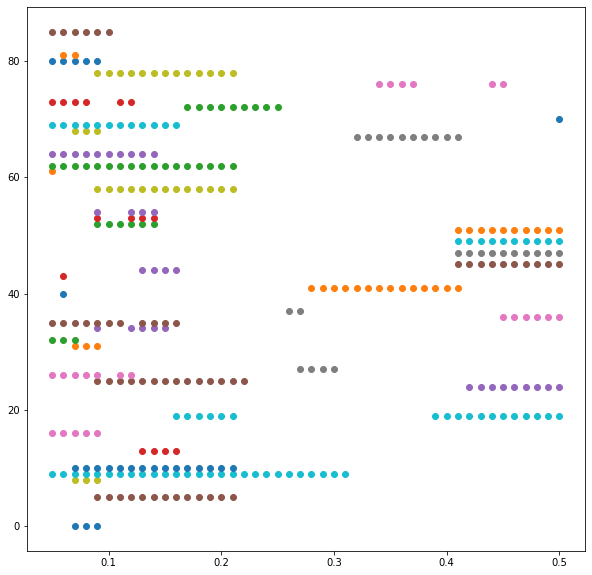
\includegraphics[width=0.95\linewidth, left]{fig/graph.png}
            };
            \node[below=of img, node distance=0cm, yshift=1cm,font=\color{red}] {Threshold value (no unit)};
            \node[left=of img, node distance=0cm, rotate=90, anchor=center,yshift=-0.8cm,font=\color{red}] {Web page};
        \end{tikzpicture}
        
        \caption{With list elements.}
        \label{fig:results-with-list}
        
    \end{subfigure}
    %
    \begin{subfigure}[b]{.49\textwidth}
        \begin{tikzpicture}[right]
            \node(img){
             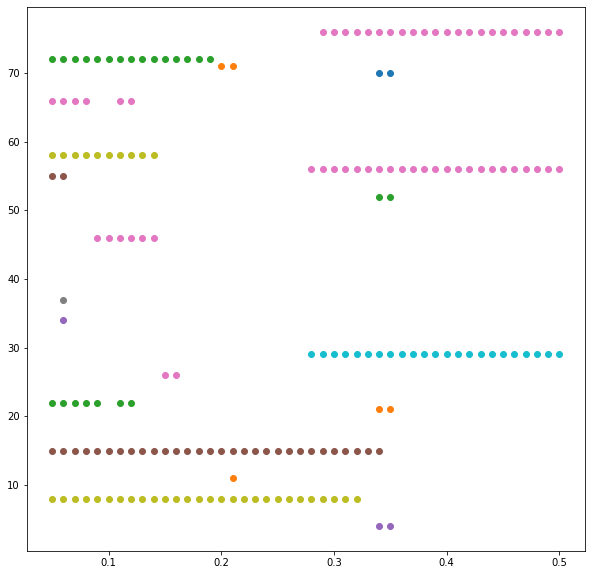
\includegraphics[width=0.95\linewidth, right]{fig/withou-list.png}
            };
            \node[
                below=of img, node distance=0cm, yshift=1cm, font=\color{red}
            ]{Threshold value (no unit)};
        \end{tikzpicture}
        
        \caption{Only table elements.}
        \label{fig:results-without-list}
        
    \end{subfigure}
    
    \caption{Closest results per page in a margin of $\pm 5$. Each point is a run where the number of data records is within a margin of $\pm 5$ relative to the ground truth. The x-axis is the threshold distance used for that run and the y-axis is merely for different pages.}
    \label{fig:results-in-margin}
    
\end{figure}


Notice that the margin of $\pm 5$ used for this plot is relatively loose. A large part of the pages have only a few tens of data records, so having $5$ data records identified is already bad enough. With this in mind, there are a few things to conclude from this graph:

\begin{enumerate}
    
    \item \textbf{There are many blank lines}: regardless of the threshold, the number of data records is \emph{far} from the ground truth.
    
    \item \textbf{There is no gold threshold}: the authors of MDR claim to achieve very high accuracy with a threshold of $0.30$. Here we see that no value is capable of having relevant results in most of the pages. If it was the case, there would be a visible vertical line or column full of dots.
    
    \item \textbf{The sensitivity varies enormously}: we can see pages where the value of the threshold seems to not even matter, while, for others, there is are very few (or even one) values with relevant results. 
    
\end{enumerate}

Therefore, we can see from Figure \ref{fig:results-with-list} that MDR does not perform well overall. More rigorously, the graph tells us that it \emph{probably} is not working well. I further inspected those pages using a smaller margin and a few random ones and the algorithm does not correctly find the data regions. For many of the cases where the number of data records coincides with the ground truth, the algorithm is capturing menus, sidebars, and button panels on the web pages.



\section{Conclusion}
% would have chosen another framework if I knew the id issue...

My implementation of the Mining Data Records (MDR) ended up being rather correct in terms of software engineering, but the algorithm simply does not properly work on today's pages anymore. I can see two clear improvements that could be useful for the code structure itself: (1) replacing \path{lxml} and (2) implementing more unit tests. 

Although \path{lxml} has useful features and does fit well most of the needs of the project, it introduced the problem with nodes identification (explained in Section \say{\nameref{txt:classes}}). This issue consequently introduced the need for another solution that is not clean and makes the implementation stateful.

The unit tests showed to be very handy to debug my code as I iteratively made modifications to my code. It would probably be useful to have some examples a bit more complex in the core functions. The module \path{files_management} has some important functionalities that make it easier to manipulate the core code, so it would be useful to have unit tests for it as well.

As shown in the results, unfortunately, this algorithm does not perform well on modern pages regardless of the parameters used. This work could further be improved by investigating the local behavior of the algorithm. If we verify that it is indeed possible to still use MDR with data records embedded in lists, it could be possible to make it work. For instance, by tweaking the \path{minimum_depth} it could be possible to get rid of the menus and panels.


% %%%%%%%%%%%%%%%%%%%%%%%%%   REFS   %%%%%%%%%%%%%%%%%%%%%%%%%%%%%%%%%
\newpage
\bibliography{refs} 


\end{document}